% IMPORTANTE:
% Para poner barrabaja en una url hay que cambiar '_' por '\textunderscore'

\documentclass[a4paper,12pt,oneside]{book}

% Paquetes
\usepackage[spanish]{babel} % Indicar idioma español
\usepackage[utf8]{inputenc} % Poder poner tildes directamente
\usepackage{graphicx} % Para imcuir gráficos
\usepackage{cite} % Para crear referencias
\usepackage{svg} % Para usar imágenes en formato vectorial
\usepackage{float} % Para modificar como aparecen las imagenes
\usepackage{listings} % Para introducir código
\usepackage{times}
\usepackage{color} % para añadir colores
\usepackage{hyperref}  % Para que se creen enlaces en el documento (a otras partes o a la web)
\usepackage{AnonymousPro}
\usepackage{url}

% Estilo
% Estilo
\renewcommand{\familydefault}{\sfdefault} % Cambia la tipografía de todo el documento
\setlength{\parskip}{2mm} % Define la distancia entre parrafos (por defecto = 0)

% Estilo de los enlaces
\hypersetup{
	colorlinks,
	citecolor=black,
	filecolor=black,
	linkcolor=black,
	urlcolor=black
}

% -- ESTILO PARA EL CODIGO -------------------------------------------
\definecolor{gray95}{gray}{.95}
\definecolor{gray85}{gray}{.80}
\definecolor{gray45}{gray}{.45}
\definecolor{myturquoise}{RGB}{0, 128, 128}

\lstset{ 
	frame=Ltb,
	framerule=0pt,
	aboveskip=0.5cm,
	framextopmargin=3pt,
	framexbottommargin=3pt,
	framexleftmargin=0.2cm,
	framesep=0pt,
	rulesep=2.0pt,
	backgroundcolor=\color{gray95},
	rulesepcolor=\color{black},
	%
	stringstyle=\ttfamily,
	showstringspaces = false,
	basicstyle=\small\ttfamily,
	commentstyle=\color{gray45},
	keywordstyle=\bfseries,
	%
	numbers=left,
	numbersep=15pt,
	numberstyle=\tiny,
	numberfirstline = false,
	breaklines=true,
}

% Minimizar fragmentado de listados
\lstnewenvironment{listing}[1][]
{\lstset{#1}\pagebreak[0]}{\pagebreak[0]}

% Estilo de codigo para la consola
\lstdefinestyle{consola}{
	language=bash,
	breaklines=true,
	basicstyle=\footnotesize\bf\ttfamily,
	backgroundcolor=\color{gray85},
	rulesepcolor=\color{myturquoise},
	numbers=none,
}

% -- FIN ESTILO PARA EL CODIGO ---------------------------------------

% Información del documento
\title{Sistema embebido para el control de un vehículo robotizado usando ROS y Docker}
\author{Julen Aristimuño \and Ander Granado \and Joseba Ruiz}
\date{\today}


\begin{document}

\frontmatter % Define la parte inicial del libro, que suele ir compuesto por:

\maketitle % Titulo del documento
\tableofcontents % Indice de contenidos
\listoffigures % Indice de figuras


\mainmatter % Define la parte frincipal del libro, el contenido

\chapter{Introducción}

	\section{Objetivo}
	En el siguiente documento se documenta el desarrollo de un sistema virtualizado para controlar un vehículo robótico. Este sistema dispondrá de diferentes módulos que estarán conectados entre sí e interactuarán entre ellos.

\chapter{Herramientas utilizadas}

\section{Hardware}
Aunque el vehículo dispone de numeroso hardware, en esta sección solo hablaremos sobre el hardware para el cual nosotros vamos a programar. En este caso todo nuestro sistema se montará en una Raspberry pi, aunque el desarrollo del sistema lo haremos en los PCs con arquitectura x86.

	\subsection{Raspberry Pi}
	Raspberry Pi es un ordenador de placa reducida que debido a us bajo coste (35 \$) y su pequeño tamaño, es ampliamente usado en sistemas de bajo coste, sistemas embebidos o en entornos educativos. Existen dos principales modelos, la Raspberry Pi y la Raspberry Pi 2. La Raspberry Pi a su vez cuenta con 4 diferentes submodelos, el A, el A+, el B y el B+.
	
	Aunque cuenta con diferentes submodelos con diferentes especificaciones, las características generales de la Raspberry Pi son \cite{rpi-wikipedia}:
	
	\begin{itemize}
		\item SoC (System on Chip) Broadcom BCM2835:
			\begin{itemize}
				\item CPU ARM 1176JZF-S a 700 MHz single-core (familia ARM11)
				\item GPU Broadcom VideoCore IV (OpenGL ES 2.0, MPEG-2 y VC-1, 1080p30 H.264/MPEG-4 AVC3)
			\end{itemize}
		\item Memoria SDRAM: 256 MB (en el modelo A) o 512 MB (en el modelo B), compartidos con la GPU
		\item Puertos USB 2.0: 1 (en el modelo A), 2 (en el modelo B) o 4 (en el modelo B+)
		\item 10/100 Ethernet RJ-45 (en el Modelo B)
		\item Salidas de video:
			\begin{itemize}
				\item Conector RCA (PAL y NTSC)
				\item HDMI (rev1.3 y 1.4)
				\item Interfaz DSI para panel LCD
			\end{itemize}
		\item Salidas de audio:
			\begin{itemize}
				\item Conector de 3.5 mm
				\item HDMI
			\end{itemize}
		\item Puertos GPIO: 8 o 17 (en el caso de las versiones +)
	\end{itemize}
	
	El segundo modelo de Raspberry Pi, conocido como Paspberry Pi 2, añade mejoras notables con respecto a la anterior generación. Sus características básicas son:
	
	\begin{itemize}
		\item SoC Broadcom BCM2836:
			\begin{itemize}
				\item 900 MHz quad-core ARM Cortex A7
				\item GPU Broadcom VideoCore IV (OpenGL ES 2.0, MPEG-2 y VC-1, 1080p30 H.264/MPEG-4 AVC3)
			\end{itemize}
		\item 1GB memoria SDRAM, compartida con la GPU
		\item 4 puertos USB 2.0
		\item 10/100 Ethernet RJ-45
		\item Salidas de video:
		\begin{itemize}
			\item Conector RCA (PAL y NTSC)
			\item HDMI (rev1.3 y 1.4)
			\item Interfaz DSI para panel LCD
		\end{itemize}
		\item Salidas de audio:
		\begin{itemize}
			\item Conector de 3.5 mm
			\item HDMI
		\end{itemize}
		\item 17 puertos GPIO
	\end{itemize}
	

\section{Software}
Para lograr dicho objetivo anteriormente descrito, se hace uso de una serie de herramientas, entre las cuales se incluye Docker y ROS.

	\subsection{Docker}
	Docker es una plataforma abierta para aplicaciones distribuidas para desarrolladores y administradores de sistemas\cite{docker-web}. Docker automatiza el despliegue de contenidos de software proporcionando una capa adicional de abstracción y automatización de virtualización a nivel de sistema operativo en Linux \cite{docker-wikipedia}. Docker utiliza características de aislamiento de recursos del kernel de Linux, 
	
		\subsubsection{Funcionamiento de Docker}
		Docker se basa en el el principio de los contenedores. Cada contenedor consta de una serie de aplicaciones y/o librerías que se ejecutan de manera independiente del OS (Sistema Operativo) principal, pero que usan el kernel Linux del sistema operativo anfitrión. Para hacer esto se hacen uso de diferentes técnicas tales como cgroups y espacios de nombres (namespaces) para permitir que estos contenedores independientes se ejecuten dentro de una sola instancia de Linux. De esta manera se logra reducir drásticamente el consumo de recursos de hardware, a cambio de que las librerías, aplicaciones o sistemas operativos deban ser compatibles con linux y ser compatibles con la arquitectura del hardware en la que se están ejecutando (x86, ARM, SPARC,...).
		
		Mediante el uso de contenedores, los recursos pueden ser aislados, los servicios restringidos, y se otorga a los procesos la capacidad de tener una visión casi completamente privada del sistema operativo con su propio identificador de espacio de proceso, la estructura del sistema de archivos, y las interfaces de red. Los contenedores comparten el mismo kernel, pero cada contenedor puede ser restringido a utilizar sólo una cantidad definida de recursos como CPU, memoria y E/S. \cite{docker-wikipedia}.

	\subsection{ROS}
	ROS (Robot Operating System) es un framework flexible para desarrollar software para robots. Es una colección de herramientas, librerías que tratan de simplificar la creación de aplicaciones complejas y robustas para todo tipo de sistemas robóticos \cite{ros-web}.
	
	ROS provee los servicios estándar de un sistema operativo tales como abstracción del hardware, control de dispositivos de bajo nivel, implementación de funcionalidad de uso común, paso de mensajes entre procesos y mantenimiento de paquetes. Está basado en una arquitectura de grafos donde el procesamiento toma lugar en los nodos que pueden recibir, mandar y multiplexar mensajes de sensores, control, estados, planificaciones y actuadores, entre otros \cite{ros-wikipedia}.


	Las áreas que incluye ROS son:
	\begin{itemize}
		\item Un nodo principal de coordinación.
		\item Publicación o subscripción de flujos de datos: imágenes, estéreo, láser, control, actuador, contacto, etc.
		\item Multiplexación de la información.
		\item Creación y destrucción de nodos.
		\item Los nodos están perfectamente distribuidos, permitiendo procesamiento distribuido en múltiples núcleos, multiprocesamiento, GPUs y clústeres.
		Login.
		\item Parámetros de servidor.
		\item Testeo de sistemas.
	\end{itemize}

\chapter{Docker}
Tras haber explicado anteriormente a grandes rasgos el funcionamiento de Docker, es conveniente antes de lanzarnos a la creación del sistema saber como crear y configurar los contenedores de Docker que conformarán el sistema. En este capítulo se explicará como empezar a trabajar con Docker, desde instalarlo y como empezar a usarlo hasta como se usan los Dockerfiles para lanzar contenedores personalizados.

	\section{Instalación}
	Lo primero que haremos será instalar Docker en nuestro sistema. En nuestro caso tenemos un sistema Ubuntu instalado en una máquina virtual, ya que nuestro hardware cuenta con SO Windows. Instalar Docker en cualguier distribución basada en Debian es tan sencillo como seguir los siguientes pasos \cite{docker-install}:
	
	\lstset{language=bash, breaklines=true, basicstyle=\footnotesize}
	\begin{enumerate}
		\item Comprobar si tenemos curl instalado
		\begin{lstlisting}[style=consola]
$ which curl
		\end{lstlisting}
		En caso de que no este instalado, instalarlo mediante:
		\begin{lstlisting}[style=consola]
$ sudo apt-get update
$ sudo apt-get install curl
		\end{lstlisting}
		\item Instalar Docker mediante el siguiente comando:
		\begin{lstlisting}[style=consola]
$ curl -sSL https://get.docker.com/ | sh
		\end{lstlisting}
		\item Comprobar que Docker se ha instalado correctamente.
		\begin{lstlisting}[style=consola]
$ docker run hello-world
		\end{lstlisting}
			Si ejecutamos el comando anterior y nos muestra información sobre Docker, ya hemos terminado de instalar Docker.
	\end{enumerate}
	
	\section{Uso básico de Docker}
	Para hacer uso de Docker necesitamos trabajar desde la terminal. La forma básica para trabajar con Docker es la siguiente:
	
	\begin{lstlisting}[style=consola]
$ docker [subcomando de docker] [parametros]
	\end{lstlisting}

	De esa manera primero indicamos que queremos usar Docker y a continuación indicamos que es lo que queremos hacer. En el ejemplo anterior hemos usado \textit{run} para ejecutar un contenedor de Docker. Por último introducimos los diferentes parámetros. La lista completa de comandos que acepta Docker se puede ver de las siguiente manera:
	% basicstyle=\scriptsize
	\begin{lstlisting}[style=consola,numbers=left]
$ docker --help
Usage: docker [OPTIONS] COMMAND [arg...]
docker daemon [ --help | ... ]
docker [ --help | -v | --version ]

A self-sufficient runtime for containers.

Options:

--config=~/.docker              Location of client config files
-D, --debug=false               Enable debug mode
-H, --host=[]                   Daemon socket(s) to connect to
-h, --help=false                Print usage
-l, --log-level=info            Set the logging level
--tls=false                     Use TLS; implied by --tlsverify
--tlscacert=~/.docker/ca.pem    Trust certs signed only by this CA
--tlscert=~/.docker/cert.pem    Path to TLS certificate file
--tlskey=~/.docker/key.pem      Path to TLS key file
--tlsverify=false               Use TLS and verify the remote
-v, --version=false             Print version information and quit

Commands:
attach    Attach to a running container
build     Build an image from a Dockerfile
commit    Create a new image from a container's changes
cp        Copy files/folders from a container to a HOSTDIR or to STDOUT
create    Create a new container
diff      Inspect changes on a container's filesystem
events    Get real time events from the server
exec      Run a command in a running container
export    Export a container's filesystem as a tar archive
history   Show the history of an image
images    List images
import    Import the contents from a tarball to create a filesystem image
info      Display system-wide information
inspect   Return low-level information on a container or image
kill      Kill a running container
load      Load an image from a tar archive or STDIN
login     Register or log in to a Docker registry
logout    Log out from a Docker registry
logs      Fetch the logs of a container
pause     Pause all processes within a container
port      List port mappings or a specific mapping for the CONTAINER
ps        List containers
pull      Pull an image or a repository from a registry
push      Push an image or a repository to a registry
rename    Rename a container
restart   Restart a running container
rm        Remove one or more containers
rmi       Remove one or more images
run       Run a command in a new container
save      Save an image(s) to a tar archive
search    Search the Docker Hub for images
start     Start one or more stopped containers
stats     Display a live stream of container(s) resource usage statistics
stop      Stop a running container
tag       Tag an image into a repository
top       Display the running processes of a container
unpause   Unpause all processes within a container
version   Show the Docker version information
wait      Block until a container stops, then print its exit code

Run 'docker COMMAND --help' for more information on a command.
	\end{lstlisting}
	
	Como se puede observar existen diferentes comandos que nos permitirán configurar Docker, obtener información sobre el y tratar con las imágenes y los contenedores de Docker. A continuación vamos a explicar algunos de ellos para poder empezar a trabajar con Docker. 
	
	El comando esencial para empezar a trabajar con Docker es el comando \textbf{\emph{run}}. Para poder lanzar directamente un contenedor de Docker, se usa el comando \textit{run}.
	
	\begin{lstlisting}[style=consola]
$ docker run ubuntu:trusty
	\end{lstlisting}
	
	Con el comando anterior hemos lanzado un contenedor de Docker que lleva Ubuntu. Lo primero que hace Docker para lanzar una imagen es comprobar si ya tiene en local la imagen desde la que se va a crear el contenedor. En caso de no tenerla accederá a unos repositorios llamados Docker Hub, donde se encuentran una gran cantidad de \textbf{\emph{Dockerfiles}}. Los \emph{Dockerfiles} son los archivos que sirven para generar esas imágenes (veremos más adelante como funcionan estos archivos especiales). Una vez Docker genere la imagen a partir del \textit{Dockerfile} ejecutará el contenedor, que a grandes rasgos es una instancia de la imagen.
	
	Podremos observar los contenedores Docker que tenemos lanzados mediante el comando \textbf{\emph{ps}} de Docker.
	
	\begin{lstlisting}[style=consola,numbers=left]
$ docker ps
CONTAINER ID        IMAGE               COMMAND                  CREATED             STATUS              PORTS               NAMES
	\end{lstlisting}
	
	Aunque hemos lanzado un contenedor, mediante el comando \emph{ps} de Docker vemos que en realidad no hay ningún contenedor en ejecución. Esto es porque los contenedores de Docker solo se mantienen activos mientras el comando con el que se han iniciado este activo \cite{docker-run}. Para poder observar el comportamiento del comando \emph{ps}, vamos a crear un contenedor demonizado, un contenedor que se ejecutará indefinidamente hasta que lo paremos. Lo haremos de la siguiente manera.
	
	\begin{lstlisting}[style=consola]
$ docker run -d ubuntu:14.04 /bin/sh -c "while true; do echo hello world; sleep 1; done"
	\end{lstlisting}
	
	Con el \textbf{-d} lo que logramos es que se siga ejecutando el contenedor en segundo plano, como si fuera un demonio (daemon), un proceso que esta siempre en ejecución. También debemos darle algo para hacer, ya que si no, tal y como hemos comentado antes, finalizará la ejecución. Esto lo logramos mediante un bucle infinito en shell script, que es lo que pasamos como parámetro entre comillas. Si ahora ejecutamos el comando \emph{ps}, comprobaremos que tenemos una máquina en ejecución.
	
	\begin{lstlisting}[style=consola,numbers=left]
$ docker ps
CONTAINER ID        IMAGE               COMMAND                  CREATED             STATUS              PORTS               NAMES
40f5c913912e        ubuntu              "/bin/sh -c 'while tr"   2 seconds ago       Up 2 seconds                            adoring_euclid
	\end{lstlisting}
	
	En caso de que queramos obtener más información sobre un contenedor de Docker, podemos usar el comando \textbf{\emph{inspect}} de Docker. La forma más básica de trabajar con este comando es la de utilizar como parámetro el ID o nombre de la maquina. Este comando nos devolverá por la salida estándar un JSON con una gran cantidad de parámetros que nos indican diferentes aspectos sobre el contenedor. También se pueden obtener solo un parámetro o un grupo de parámetros en concreto. En el siguiente ejemplo se muestra su uso, para obtener toda la información y para obtener un dato, en este caso la dirección IP del contenedor.
	
	\begin{lstlisting}[style=consola,numbers=left]
$ docker inspect adoring_euclid
# ...
# ... Se omite la salida por ser demasiado grande
# ...
$ docker inspect --format='{{.NetworkSettings.IPAddress}}' adoring_euclid
172.17.0.3
	\end{lstlisting}

	En caso de que queramos matar un contenedor, podremos hacerlo mediante el comando \textbf{\emph{stop}} o mediante el comando \textbf{\emph{kill}} de Docker. El primero mata directamente el contenedor, de manera análoga al kill de linux, a diferencia del otro, que detiene la ejecución de una manera más segura.
	
	\begin{lstlisting}[style=consola,numbers=left]
$ docker ps
CONTAINER ID        IMAGE               COMMAND                  CREATED             STATUS              PORTS               NAMES
40f5c913912e        ubuntu              "/bin/sh -c 'while tr"   2 seconds ago       Up 2 seconds                            adoring_euclid
$ docker stop 40f5c913912e
40f5c913912e
$ docker ps
CONTAINER ID        IMAGE               COMMAND                  CREATED             STATUS              PORTS               NAMES

	\end{lstlisting}
	
	Otro comando útil a la hora de gestionar Docker es el comando \textbf{\emph{images}}. El comando \textit{images} nos muestra todas las imágenes que tenemos en local. Si queremos eliminar alguna, usamos el comando \textbf{\emph{rmi}}.
	
	\begin{lstlisting}[style=consola,numbers=left]
$ docker images
REPOSITORY          TAG                 IMAGE ID            CREATED             VIRTUAL SIZE
ubuntu              latest              a005e6b7dd01        18 hours ago        188.4 MB
ros                 latest              67110eef39cf        7 weeks ago         826.7 MB
hello-world         latest              af340544ed62        9 weeks ago         960 B
$ docker rmi -f hello-world
Untagged: hello-world:latest
Deleted: af340544ed62de0680f441c71fa1a80cb084678fed42bae393e543faea3a572c
Deleted: 535020c3e8add9d6bb06e5ac15a261e73d9b213d62fb2c14d752b8e189b2b912
$ docker images
REPOSITORY          TAG                 IMAGE ID            CREATED             VIRTUAL SIZE
ubuntu              latest              a005e6b7dd01        18 hours ago        188.4 MB
ros                 latest              67110eef39cf        7 weeks ago         826.7 MB
	\end{lstlisting}
	
	\section{Creación de Dockerfiles}
	Hasta ahora hemos visto que podemos crear contenedores Docker de una manera sencilla, pero si queremos hacer algún tipo de cambio en la configuración de estos contenedores debemos hacerlo de manera manual, accediendo a la terminal del contenedor y usando comandos. Docker provee un potentísimo sistema que nos permite automatizar las tareas de configuración de nuestras imágenes de Docker, que es el uso de Dockerfiles. En realidad, cuando nosotros llamamos al comando run de Docker y no tenemos una imagen de Docker, lo que estamos haciendo es llamar a un Dockerfile que se encuentra en el Docker Hub, y mediante él generar la imagen desde la que se creará el contenedor. De esta manera, mediante el uso de imágenes personalizadas, crearemos contenedores personalizados, con programas instalados o diferentes configuraciones realizadas en ellos.
	
	Los Dockerfile tienen una sintaxis especial, que nos permitirán entre otras cosas, ejecutar comandos de linux para configurar aspectos de nuestro contenedor. A continuación se muestra el Dockerfile que se usa para crear una imagen de Ubuntu \cite{ubuntu-dockerfile}.
	
	\begin{lstlisting}[style=consola,numbers=left]
FROM scratch
ADD ubuntu-trusty-core-cloudimg-amd64-root.tar.gz /

# a few minor docker-specific tweaks
# see https://github.com/docker/docker/blob/master/contrib/mkimage/debootstrap
RUN echo '#!/bin/sh' > /usr/sbin/policy-rc.d \
&& echo 'exit 101' >> /usr/sbin/policy-rc.d \
&& chmod +x /usr/sbin/policy-rc.d \
\
&& dpkg-divert --local --rename --add /sbin/initctl \
&& cp -a /usr/sbin/policy-rc.d /sbin/initctl \
&& sed -i 's/^exit.*/exit 0/' /sbin/initctl \
\
&& echo 'force-unsafe-io' > /etc/dpkg/dpkg.cfg.d/docker-apt-speedup \
\
&& echo 'DPkg::Post-Invoke { "rm -f /var/cache/apt/archives/*.deb /var/cache/apt/archives/partial/*.deb /var/cache/apt/*.bin || true"; };' > /etc/apt/apt.conf.d/docker-clean \
&& echo 'APT::Update::Post-Invoke { "rm -f /var/cache/apt/archives/*.deb /var/cache/apt/archives/partial/*.deb /var/cache/apt/*.bin || true"; };' >> /etc/apt/apt.conf.d/docker-clean \
&& echo 'Dir::Cache::pkgcache ""; Dir::Cache::srcpkgcache "";' >> /etc/apt/apt.conf.d/docker-clean \
\
&& echo 'Acquire::Languages "none";' > /etc/apt/apt.conf.d/docker-no-languages \
\
&& echo 'Acquire::GzipIndexes "true"; Acquire::CompressionTypes::Order:: "gz";' > /etc/apt/apt.conf.d/docker-gzip-indexes

# enable the universe
RUN sed -i 's/^#\s*\(deb.*universe\)$/\1/g' /etc/apt/sources.list

# overwrite this with 'CMD []' in a dependent Dockerfile
CMD ["/bin/bash"]
	\end{lstlisting}

	Se puede observar que hay diferentes comandos en mayúscula que llaman la atención. Estos comandos son los que reconoce Docker. Con el comando \textbf{FROM} se le indica a Docker otro Dockerfile sobre el que empezar, en caso de que queramos partir de una imagen ya existente. En este caso al usar el termino \textit{scratch}, se le indica que parta desde cero. Es \emph{obligatorio} empezar siempre un Dockerfile con este comando.
	
	Con el comando \textbf{ADD}, se añade un archivo, indicándole dónde queremos añadirlo. En este caso añade un \textit{tarball} en el que se encuentra Ubuntu. Con el comando \textbf{RUN}, se ejecuta un comando de linux. El Dockerfile de Ubuntu utiliza una serie de comandos para realizar diversas tareas, como definir repositorios. Con el comando \textbf{CMD}, se define un comportamiento por defecto a la hora de lanzar la imagen, en el caso de Ubuntu se lanza una terminal en bash.
	
	Existen más comandos que soportan los Dockerfiles. La lista de todos los comandos que permite Un Dockerfile es la siguiente \cite{dockerfiles-doc}:
	\begin{itemize}
		 \item \textbf{FROM}: Indica que Dockerfile tomar como base (\textit{scratch} para no usar ninguno)
		 \item \textbf{MAINTAINER}: Indica quien es el encargado me mantener el Dockerfile. Normalmente se usa un nombre o una dirección de correo electrónico
		 \item \textbf{RUN}: Sirve para ejecutar comandos
		 \item \textbf{CMD}: Sirve para establecer la acción por defecto al lanzar un contenedor. Solo se puede usar una ver en un Dockerfile
		 \item \textbf{LABEL}: Sirve para añadir metadatos a una imagen
		 \item \textbf{EXPOSE}: Sirve para indicar al contenedor que puertos tiene que estar escuchando
		 \item \textbf{ENV}: Sirve para crear variables de entorno
		 \item \textbf{ADD}: Sirve para copiar archivos al contenedor. Permite usar URLs externas y descomprime archivos automáticamente
		 \item \textbf{COPY}: Permite copiar archivos en local al contenedor.
		 \item \textbf{ENTRYPOINT}: Permite configurar un contenedor para ejecutarlo como un ejecutable 
		 \item \textbf{VOLUME}: Sirve para crear puntos de montaje dentro de un contenedor
		 \item \textbf{USER}: Sirve para configurar el nombre de usuario o UID que se va a usar para ejecutar las instrucciones que le suceden en el Dockerfile
		 \item \textbf{WORKDIR}: Sirve para configurar el directorio con respecto al que se van a ejecutar las instrucciones que le suceden en el Dockerfile
		 \item \textbf{ONBUILD}: Sirve para definir instrucciones que se van a ejecutar en caso de usarse el Dockerfile como base para otro Dockerfile
	\end{itemize}
	
	\section{Profundizar en Docker}
	Aunque hemos explicado lo básico sobre docker, no es el objetivo de este documento explicar el funcionamiento al detalle de Docker ni ser una guía de referencia a la hora de empezar a usarlo. En caso de que se quiera conocer el funcionamiento de todos los comandos de docker, la gestión de las imágenes de Docker, o se quiera obtener más información del Docker Hub, en la documentación oficial de Docker \cite{docker-docs} se puede encontrar todo lo necesario para comprender al detalle el funcionamiento de Docker.
	
	Tras haber explicado el funcionamiento básico de Docker y algunos puntos para poder iniciarnos con él, a continuación profundizaremos en el tema de las redes en Docker, un tema esencia para poder lanzarnos a construir nuestro sistema.

\chapter{Nerworking en Docker}
Con Docker podemos crear una gran cantidad de contenedores diferentes que se ejecuten de manera simultánea. Es lógico que a la hora de crear un sistema nos interese comunicar los contenedores entre ellos para que puedan transmitirse información. Como vamos a construir un sistema de paso mensajes entre contenedores con ROS (cómo usaremos ROS lo veremos en el siguiente capítulo) necesitamos crear una red entre esos contenedores. Para ello, en este capítulo se explicaran diferentes conceptos sobre configuración de redes en Docker.

	\section{\textit{docker0}}
	Lo primero que hay que saber es que al iniciarse Docker, por defecto, se crea en el anfitrión (host) una interfaz virtual que tiene como nombre \textbf{\emph{docker0}} \cite{docker-network-advanced}. Docker coge de manera aleatoria una dirección IP y una subred de rango privado y se la asigna a \emph{docker0}. Las direcciones MAC de los contenedores se asignan usando la dirección IP de canda contenedor, para evitar de esta manera colisiones ARP.
	
	Lo que hace especial a \emph{docker0}, es que no solo es una interfaz, sino que es un puente Ethernet virtual que redirige automáticamente los paquetes entre cualquier otra interfaz que esté conectada a él. De esta manera se pueden comunicar tanto los contenedores entre ellos como con el host.
	
	Además desde un contenedor también se puede acceder a internet. En el capítulo anterior lanzamos contenedores que se creaban mediante los Dockerfiles que se obtenían del Docker Hub, que es un servidor web que se encuentra en internet. 
	
	Sin embargo, \textbf{no} podemos acceder a los contenedores desde fuera, desde internet. Por defecto está 
	establecido así, principalmente por temas de seguridad, aunque obviamente se puede cambiar.
	
	\section{Ping entre contenedores}
	Si todos los contenedores que creamos se encuentran en una misma subred, podemos comunicarnos entre ellos simplemente con sus direcciones IP privadas o sus nombres de red. La forma más sencilla para probar la comunicación entre dos sistemas es el uso de la herramienta ping de linux.
	
	Vamos a lanzar por una parte dos contenedores Docker en dos terminales separadas. Para esta prueba usaremos la misma imagen que vamos a usar para crear nuestro sistema, que es la imagen \emph{osrf/ros:indigo-desktop}, a la que previamente hemos hecho un \emph{pull} para tenerla generada, ya que ocupa alrededor de 1,6 GB. Creamos los contenedores de la siguiente manera.
	
	\begin{lstlisting}[style=consola]
$ docker run -it osrf/ros:indigo-desktop /bin/bash
	\end{lstlisting}
	
	Desde fuera comprobamos que tenemos los contenedores en ejecución.
	
	\begin{lstlisting}[style=consola,numbers=left]
$ docker ps
CONTAINER ID        IMAGE                     COMMAND                  CREATED             STATUS              PORTS               NAMES
829a49bb2cfa        osrf/ros:indigo-desktop   "/ros_entrypoint.sh /"   6 seconds ago       Up 6 seconds                            compassionate_mccarthy
2f3c19da0cb8        osrf/ros:indigo-desktop   "/ros_entrypoint.sh /"   16 seconds ago      Up 16 seconds                           grave_mahavira
	\end{lstlisting}
	
	Podemos obtener la dirección IP de un contenedor tanto desde fuera como desde dentro de Docker. En este caso lo haremos desde fuera mediante el \emph{inspect} de Docker.
	
	\begin{lstlisting}[style=consola,numbers=left]
$ docker inspect --format='{{.NetworkSettings.IPAddress}}' compassionate_mccarthy
172.17.0.5
$ docker inspect --format='{{.NetworkSettings.IPAddress}}' grave_mahavira
172.17.0.4
	\end{lstlisting}
	
	Ya tenemos las direcciones IP privadas que genera \emph{docker0} para los dos contenedores. Ahora probamos a hacer un ping desde un contenedor a otro. Desde el contenedor \textit{grave\_mahavira} con IP 172.17.0.4 al contenedor \textit{compassionate\_mccarthy} con IP 172.17.0.5 se haría así.
	
	\begin{lstlisting}[style=consola,numbers=left]
root@2f3c19da0cb8:/# ping 172.17.0.5
PING 172.17.0.5 (172.17.0.5) 56(84) bytes of data.
64 bytes from 172.17.0.5: icmp_seq=1 ttl=64 time=0.085 ms
64 bytes from 172.17.0.5: icmp_seq=2 ttl=64 time=0.058 ms
64 bytes from 172.17.0.5: icmp_seq=3 ttl=64 time=0.061 ms
64 bytes from 172.17.0.5: icmp_seq=4 ttl=64 time=0.060 ms
64 bytes from 172.17.0.5: icmp_seq=5 ttl=64 time=0.106 ms
64 bytes from 172.17.0.5: icmp_seq=6 ttl=64 time=0.135 ms
^C
--- 172.17.0.5 ping statistics ---
6 packets transmitted, 6 received, 0% packet loss, time 4997ms
rtt min/avg/max/mdev = 0.058/0.084/0.135/0.028 ms
	\end{lstlisting}
	
	Se puede hacer exactamente lo mismo con los nombres de los contenedore docker ya que esto son los nombres que se le dan en la red \emph{docker0} a la que están conectados. En este caso haremos un ping desde \textit{compassionate\_mccarthy} a \textit{grave\_mahavira} usando para ello el nombre del contenedor.
	
	\begin{lstlisting}[style=consola,numbers=left]
root@829a49bb2cfa:/# ping grave_mahavira
PING grave_mahavira (172.17.0.4) 56(84) bytes of data.
64 bytes from grave_mahavira.bridge (172.17.0.4): icmp_seq=1 ttl=64 time=0.087 ms
64 bytes from grave_mahavira.bridge (172.17.0.4): icmp_seq=2 ttl=64 time=0.066 ms
64 bytes from grave_mahavira.bridge (172.17.0.4): icmp_seq=3 ttl=64 time=0.066 ms
64 bytes from grave_mahavira.bridge (172.17.0.4): icmp_seq=4 ttl=64 time=0.067 ms
64 bytes from grave_mahavira.bridge (172.17.0.4): icmp_seq=5 ttl=64 time=0.066 ms
64 bytes from grave_mahavira.bridge (172.17.0.4): icmp_seq=6 ttl=64 time=0.064 ms
^C
--- grave_mahavira ping statistics ---
6 packets transmitted, 6 received, 0% packet loss, time 5001ms
rtt min/avg/max/mdev = 0.064/0.069/0.087/0.010 ms
	\end{lstlisting}
	
	Debido a esto, los nombres que se usan en los contendores deben ser \textbf{únicos}. Debemos tenerlo en cuanta a la hora de renombrar los contenedores. Tampoco podemos cambiar el nombre de un  contenedor durante su ejecucíon, solo podremos nombrarlo al lanzarlo.
	
	\section{Links entre contenedores}
	Como hemos visto, a causa de tener los contenedores dentro de una red privada, comunicarlos entre ellos es algo trivial. El problema de transmitir información de esta manera es que el interfaz \emph{docker0} se usa para \textbf{todos} los contenedores que estén en ejecución en ese host. Si queremos realizar una comunicación privada entre dos contenedores, que sea invisible para el resto de contenedores, debemos usar el mecanismo que provee Docker, el linkado de contenedores \cite{docker-network-linking}.
	
	Docker provee también un sistema para mapear puertos entre dos contenedores, aunque el mejor sistema que podemos usar para conectar contendores el el linkado, ya que abstrae todo el sistema de puertos, y crea un puente virtual que permite una comunicación segura entre los contenedores.
	
	Para usar el sistema de links de Docker, debemos usar el flag \textbf{--link} a la hora de lanzar el contenedor. Primero vamos a crear un contenedor al que llamaremos ros1.
	
	\begin{lstlisting}[style=consola]
$ docker run -it --name ros1 osrf/ros:indigo-desktop /bin/bash
	\end{lstlisting}
	
	A continuación vamos a crear otro contenedor, al que llamaremos \emph{ros2}, que este linkado a \emph{ros1}.
	
	\begin{lstlisting}[style=consola]
$ docker run -it --name ros2 --link ros1 osrf/ros:indigo-desktop /bin/bash
	\end{lstlisting}
	
	Ahora desde fuera de los contenedores, miramos los links que tiene \emph{ros2} mediante \emph{inspect}.
	
	\begin{lstlisting}[style=consola,numbers=left]
$ docker inspect -f "{{ .HostConfig.Links }}" ros2
[/ros1:/ros2/ros1]
	\end{lstlisting}
	
	Ahora desde \emph{ros2} podemos acceder a la información de \emph{ros1}.
	
	Para lograr este enlace Docker usa dos sistemas diferentes:
	
	\begin{itemize}
		\item Variables de entorno
		\item Actualizar el fichero \emph{/etc/hosts}
	\end{itemize}
	
	Todo esto lo realiza de manera automática a la hora de enlazar dos contenedores.
	
	\section{\textit{network} de Docker}
	
	\textit{\footnotesize \textbf{NOTA:} el contenido de toda esta sección se basa en la versión de la rama experimental de Docker. A día de hoy (27 de octubre de 2015) esta funcionalidad no se encuentra en la versión estable de Docker, que es la 1.8.3. La versión utilizada para la explicación es la versión 1.9.0-dev (build b92df9f), de la rama de desarrollo.}

	En la rama experimental de Docker, se encuentra una funcionalidad que lleva gestándose desde que salió la versión 1.7 de Docker. Esta nueva funcionalidad permite crear redes con diferentes topologías de una manera sencilla, abstrayendo de configuraciones, al igual que los links de Docker. A diferencia de los links de Docker, que está más orientados a conectar directamente contenedores, esta nueva función permite crear redes virtuales enteras.
	
	La forma de trabajar con esta funcionalidad es mediante el uso del comando \textit{\emph{network}}.
	
	\begin{lstlisting}[style=consola]
$ docker network --help

Usage:	docker network [OPTIONS] COMMAND [OPTIONS]

Commands:
disconnect               Disconnect container from a network
inspect                  Display detailed network information
ls                       List all networks
rm                       Remove a network
create                   Create a network
connect                  Connect container to a network

Run 'docker network COMMAND --help' for more information on a command.

--help=false       Print usage
	\end{lstlisting}
	
	\subsection{Prueba de \textit{network} con nodos ROS}

% WORKING ON PROGRESS --------------------------------------------------------------------

	Para probar el funcionamiento del comando \emph{network}, vamos a hacer algo diferente. vamos a hacer uso de máquinas ROS pero con una serie de tutoriales instalados que no spermitirán probar el funcionamiento del comando. Para generar la imagen partiremos del siguiente Dockerfile.

	\lstinputlisting[style=consola,numbers=left]{../Dockerfiles/ros-tutorials/Dockerfile.}
	
	A partir del Dockerfile generamos la imagen de la siguiente manera.

	\begin{lstlisting}[style=consola]
$ docker build --tag ros:ros-tutorials .
	\end{lstlisting}

	A continuación vamos a crear la red. Para ello tenemos que usar el subcomando \emph{create} de \emph{network}. Lo haremos de la siguiente manera.

	\begin{lstlisting}[style=consola]
docker network create red_ros
dd9a08f95ed51940155daf4b9c2048bae3de5fbcc48a439fa88edefd775dcc52
	\end{lstlisting}
	
	Tras haber creado la red, procedemos a crear los nodos que conformarán la misma. Estos nodos serán contenedores ROS instanciados a partir de la imagen generada anteriormente.
	
	En desarrollo...
	
\iffalse
	
%Now that we have a network, we can create services. Services advertise there location on the network, making it easy to resolve the location/address of the service specific container. We'll use this make sure our ROS nodes can find and connect to our ROS master.

%Run services
%To create a container for the ROS master and advertise it's service:

	El primer nodo que crearemos será el nodo maestro (\emph{master}). Este será el que ejecute \emph{roscore}, que se necesario para que ROS funcione.

	\begin{lstlisting}[style=consola,numbers=left]
$ docker run -it --rm \
             --publish-service=master.red_ros \
             --name master \
             ros:ros-tutorials \
             roscore
	\end{lstlisting}
	
%Now you can see that master is running and is ready manage our other ROS nodes. To add our talker node, we'll need to point the relevant environment variable to the master service:

	El segundo nodo que crearemos sera uno que haga la función de generar los mensajes, conocido como \emph{talker}. Lo crearemos de la siguiente manera.
		
	\begin{lstlisting}[style=consola,numbers=left]
$ docker run -it --rm\
             --publish-service=talker.red_ros \
             --env ROS_HOSTNAME=talker \
             --env ROS_MASTER_URI=http://master:11311 \
             --name talker \
             ros:ros-tutorials \
             rosrun roscpp_tutorials talker
	\end{lstlisting}
	
%Then in another terminal, run the listener node similarly:

	Si acabamos de crear un nodo que habla, lo lógico sería crear un nodo que escuche. Este tipo de nodo será el \emph{listener}, y lo crearemos de la siguiente manera.

	\begin{lstlisting}[style=consola,numbers=left]
$ docker run -it --rm\
             --publish-service=listener.red_ros \
             --env ROS_HOSTNAME=listener \
             --env ROS_MASTER_URI=http://master:11311 \
             --name listener \
             ros:ros-tutorials \
             rosrun roscpp_tutorials listener
	\end{lstlisting}

\fi
%-----------------------------------------------------------------------------------------
	
	\section{Configuración manual de redes}
	Aunque en este capítulo se han enseñado varios mecanismos que provee Docker para administrar redes de contenedores, también podemos configurar toda nuestra red de una manera más tradicional, mediante la modificación de archivos como \emph{/etc/hosts} o \emph{/etc/interfaces} en nuestros contenedores, el uso de \emph{Iptables}, configuración de DNS,... 
	
	Docker mediante estos mecanismos busca abstraer parte de la configuración para hacerla mas sencilla de cara al desarrollador o al administrador.
	
	Prácticamente cualquier aspecto relacionado con las redes se puede configurar en Docker mediante una serie de flags especiales a la hora de lanzar el servicio de Docker, por lo que no se pueden modificar mientras Docker esté en ejecución (no confundir con que un contenedor esté en ejecución). Algunos de esos comandos con flags especiales solo se pueden ejecutar con el servicio de Docker parado. Varios de los mas importantes son.
	
	\begin{lstlisting}[style=consola,numbers=left]
--default-gateway=IP_ADDRESS # Define la IP a la que se conectaran los contenedores de Docker al crearse, por defecto se usa la de docker0
--icc=true|false # Indica si se permite la comunicacion entre contenedores, por defecto true
--ipv6=true|false # Define si se usa IPv6, por defecto false
--ip-forward=true|false # Indica si esta activada la comunicacion entre los contenedores y el exterior, por defecto true
--iptables=true|false # Define si se perminte el uso de iptables (filtra direcciones y puertos, se usa como firewall en sistemas tipo UNIX)
	\end{lstlisting}
	
	En la documentación de Networking avanzado de Docker \cite{docker-network-advanced} se puede encontrar mucha más información de como hacer esto.
	

\chapter{Creación del sistema}

El sistema que vamos a crear constara de las siguientes partes. Primero sobre las maquinas con SO Windows se instalara una maquina virtual Ubuntu sobre Virtualbox para trabajar en un entorno linux. A día de hoy existen formas de trabajar directamente con Docker en sistemas Windows tanto por CLI como a través de una interfaz gráfica, aunque estas se basan en emular el kernel de linux. Para este caso se ha optado por trabajar en un entorno linux conocido para hacer más simple el despligue del sistema.

Dentro de dicha máquina Ubuntu se instalará el propio Docker. Mediante Docker crearemos diferentes contenedores. Cada uno de esos contenedores contendrá una imagen de Ubuntu que vendrá con ROS instalado. Estas maquinas se comunicaran entre ellas mediante OpenVPN. Esta red OpenVPN sera configurada en un contenedor diferente, y sera la red a la que el resto de contenedores se conecten.

El esquema del sistema vendría a ser el que se muestra en la Figura \ref{fig:esquemaOriginal}.
\begin{figure}[H] % Con el parámetro H la imagens se muestra justo en el sitio en el que se ha definido
	\centering
	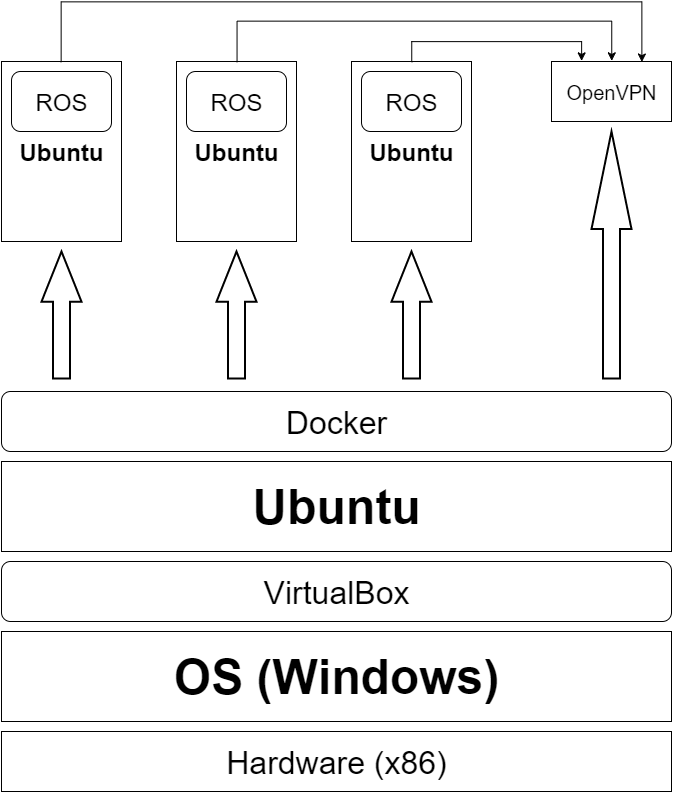
\includegraphics[width=0.8\textwidth]{figuras/esquemaOriginal}
	%		\includesvg{figuras/esquemaOriginal}
	\caption{Esquema del sistema en un ordenador x86}
	\label{fig:esquemaOriginal}
\end{figure}

Posteriormente integraremos nuestro sistema en una Raspberry Pi. El esquema del sistema aplicado en una Raspberry Pi se muestra en la Figura \ref{fig:esquemaRPi}.
\begin{figure}[H]
	\centering
	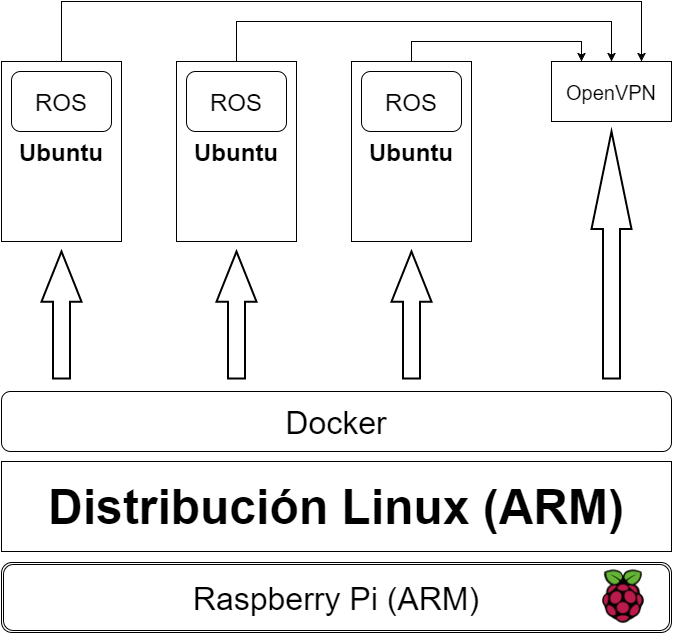
\includegraphics[width=0.8\textwidth]{figuras/esquemaRPi}
	%		\includesvg{figuras/esquemaRPi}
	\caption{Esquema del sistema en una Raspberry Pi}
	\label{fig:esquemaRPi}
\end{figure}

	

\chapter{ROS}
Anteriormente se ha explicado qué es ROS y que características tiene. En este capitulo se pasara a profundizar en su funcionamiento, y mostraremos como se pueden programar los sistemas de paso de mensajes que pasaremos a implementar en nuestro sistema de contenedores Docker anteriormente creado.




\backmatter

% Bibliografía, glosario, ...
\bibliographystyle{plainnat}
\bibliography{biblio}

\end{document}